<<<<<<< HEAD
=======
 
>>>>>>> d746ac4214360db2b50c1fa9b27a5a523f0dd66d
% -*- root: ../../main.tex -*-
\section{ECS}
\label{sec:ecs_design}
Tradizionalmente nello sviluppo di applicazioni si tende ad utilizzare un approccio di design basato sull'\textbf{ereditarietà}. Questa scelta, attraverso la crea-zione di \textbf{gerarchie semantiche} precise (Persona -> Studente), permette generalmente di ottenere implementazioni più \textbf{robuste} e \textbf{strutturate}. Nell'ambito dei videogiochi, dove è necessario un elevato grado di \textbf{flessibilità}, queste gerarchie strutturate possono risultare \textbf{costrettive}.
Al fine di eliminare questa problematica nel tempo ci si è diretti verso approcci basati maggiormente sulla \textbf{composizione}. Il pattern architetturale \texttt{ECS} nasce proprio seguendo questa filosofia di pensiero.

\subsection{Il Pattern}
\label{subsec:ecs_pattern}
Il modello \textbf{ECS} è costituito da tre parti fondamentali: entità, componenti e sistemi.
\begin{itemize}
	\item{\textbf{Entity:}} costituisce una \textbf{rappresentazione astratta} di una entità in gioco. Essa è caratterizzata in un dato momento da una serie di proprietà che possono \textit{variare liberamente}. \textit{Concettualmente}, pur avendo un aspetto \textbf{dinamico} dal punto di vista delle proprietà ad essa associate, un'entità deve rimanere \textbf{fedele} alla sua natura. 

	Per esempio un'entità nemica manterrà sempre la sua natura avversa al giocatore, pur avendo la possibilità di \textit{modificare le sue proprietà}.
	\item{\textbf{Component:}} le proprietà associate all'entità prendono il nome di \textbf{componenti}. Essi sono la vera \textbf{componente modulare} di ECS poiché possono essere \textbf{aggregati} ad ogni entità in modo \textbf{dinamico}. La loro composizione costituisce lo \textbf{stato} dell'entità a cui sono associati.
	\item{\textbf{System:}} il sistema rappresenta il vero aspetto \textbf{funzionale} di ECS poiché costituisce un \textit{modulo} dedicato unicamente alla gestione del \textbf{comportamento} delle singole entità. Il punto di forza del pattern sta nel fatto che ogni \textbf{sistema agisce} su una serie di \textbf{componenti} (in base alla tipologia), di conseguenza nel momento in cui un componente verrà rimosso da un'entità quest'ultima vedrà \textbf{modificato} il proprio comportamento.
\end{itemize}

\subsection{Approcci di Design}
Come visto in precedenza in \ref{subsec:ecs_pattern}, l'idea alla base di ECS è molto semplice, tuttavia durante il processo di \textbf{concretizzazione} alcuni aspetti concettuali vengono realizzati in modo leggermente diverso per \textit{esigenze di carattere implementativo} (performance, cache, ecc).  Dal punto di vista progettuale esistono diversi \textbf{approcci possibili}:
\begin{itemize}
	\item{\textbf{Approccio OOP:}} questa tipologia di approccio riprende l'idea che sta alla base della \textbf{programmazione ad oggetti}; in particolare viene promosso il concetto secondo il quale ogni oggetto possiede al proprio interno uno \textbf{stato} e un \textbf{comportamento}. Un ECS di tipo OOP sarà caratterizzato da entità che \textbf{contengono} i propri \textbf{componenti} e si occupano della loro \textbf{gestione}.
	\item{\textbf{Approccio Data-Driven:}} in questo caso stato e comportamento vengono mantenuti in \textbf{moduli dedicati} promuovendo una maggiore \textbf{separazione dei concetti}. L'ECS in questo caso sarà caratterizzato da \textbf{moduli di gestione} ai quali sarà delegata il \textbf{controllo} e la \textbf{connessione} di entità e componenti.
\end{itemize}

\paragraph{Alcune considerazioni di basso livello:}
Nella definizione del pattern ECS ogni sistema si occupa di gestire solamente uno o più componenti, \textbf{aggiornandoli} in blocco contemporaneamente. 

Un approccio più OOP consisterebbe nel modellare \textit{ogni entità come un oggetto} che deve implementare una sotto-interfaccia diversa in base al tipo, ereditando, di conseguenza, i metodi per l'aggiornamento. Questo causa \textbf{problemi di performance} all'aumentare delle entità da gestire, poiché ad ogni aggiornamento verrebbe caricato in \textbf{cache} l'intero oggetto aumentando così la \textbf{latenza} relativa alla fase di loading. Ciò comporta un \textbf{degradamento} importante delle \textbf{performance}.


\subsection{Design Proposto}
L'analisi delle opzioni possibili e del loro sviluppo ha portato a scegliere un approccio data-driven dato che garantisce nel complesso una maggiore \textbf{estendibilità} e \textbf{performance} migliori. L'approccio scelto inoltre si \textbf{integra} molto bene con il \textbf{paradigma funzionale} poiché permette di sfruttare al meglio le caratteristiche di quest'ultimo.

Il design finale ottenuto è quello raffigurato in \ref{fig:ECS}.

\begin{figure}[H]
	\centering
	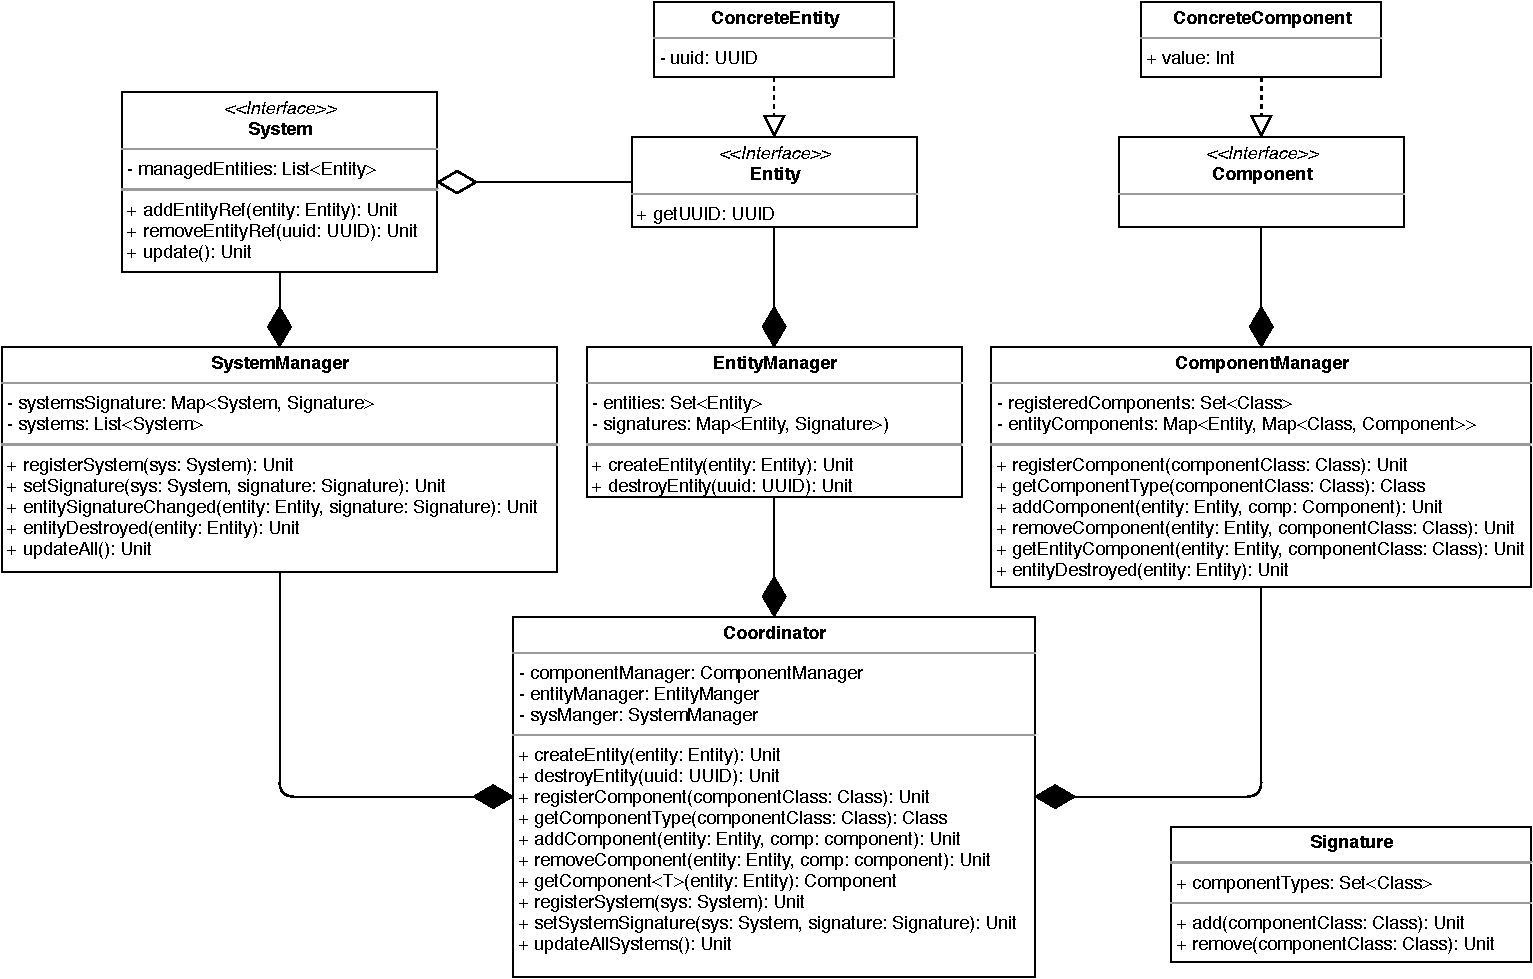
\includegraphics[width=0.99\columnwidth]{drawio/ECS/ECS.pdf}
	\caption{Diagramma di classe rappresentante il design proposto.}
	\label{fig:ECS}
\end{figure}

Come si evince dal diagramma si è scelto di utilizzare una \textbf{struttura basata su gestori} (\texttt{Manager}) ognuno responsabile di un particolare aspetto di ECS. Inoltre è stato introdotto un \textbf{punto di snodo} (\texttt{Coordinator}) con il compito di \textbf{coordinare} i vari gestori.
Di seguito verranno presentati i principali moduli presenti all'interno del diagramma:
\begin{itemize}
	\item{\textbf{Core ECS:}}
	\begin{itemize}
		\item{\textbf{Entity:}} rappresenta il concetto di entità classico di ECS. Nel nostro caso un'entità è rappresentata dalla propria \textbf{istanza di tipo} (che ne descrive la natura) e un \textbf{identificatore}.
		\item{\textbf{Component:}} rappresenta in toto il concetto di componente di ECS.
		\item{\textbf{System:}} costituisce un \textbf{modulo passivo} di gestione di entità che viene aggiornato 
		dall'esterno (\texttt{update()}). Ogni sistema è inoltre caratterizzato da una \texttt{Signature} che corrisponde ad un \textbf{insieme di componenti} gestiti.
	\end{itemize}
	\item{\textbf{Managers:}}
	\begin{itemize}
		\item{\textbf{Entity Manager:}} modulo dedicato alla gestione delle entità di gioco. Consiste in un \textbf{accentratore} per tutte le \textbf{istanze} di entità e si occupa del loro \textbf{inserimento} e \textbf{rimozione}. 
		\item{\textbf{Component Manager:}} tiene traccia delle \textbf{associazioni} fra \textbf{entità} e \textbf{componenti} e gestisce l'\textbf{aggiunta} e \textbf{rimozione} di questi ultimi.
		\item{\textbf{System Manager:}} costituisce un aggregatore di sistemi e ha lo scopo di \textbf{mantenere coerenti} i legami fra sistema, entità e componente in base alla \textbf{signature del sistema}. 
	\end{itemize}
	\item{\textbf{Coordinator:}} contiene la logica core di tutto l'ECS e ha lo scopo fondamentale di \textbf{coordinare i manager} \textbf{accentrando} le operazioni da essi fornite.
\end{itemize}


\subsection{Funzionamento}
Introdotto il design di dettaglio relativo ad ECS è necessario definirne il \textbf{funzionamento} evidenziando le interazioni.
\begin{figure}[H]
	\centering
	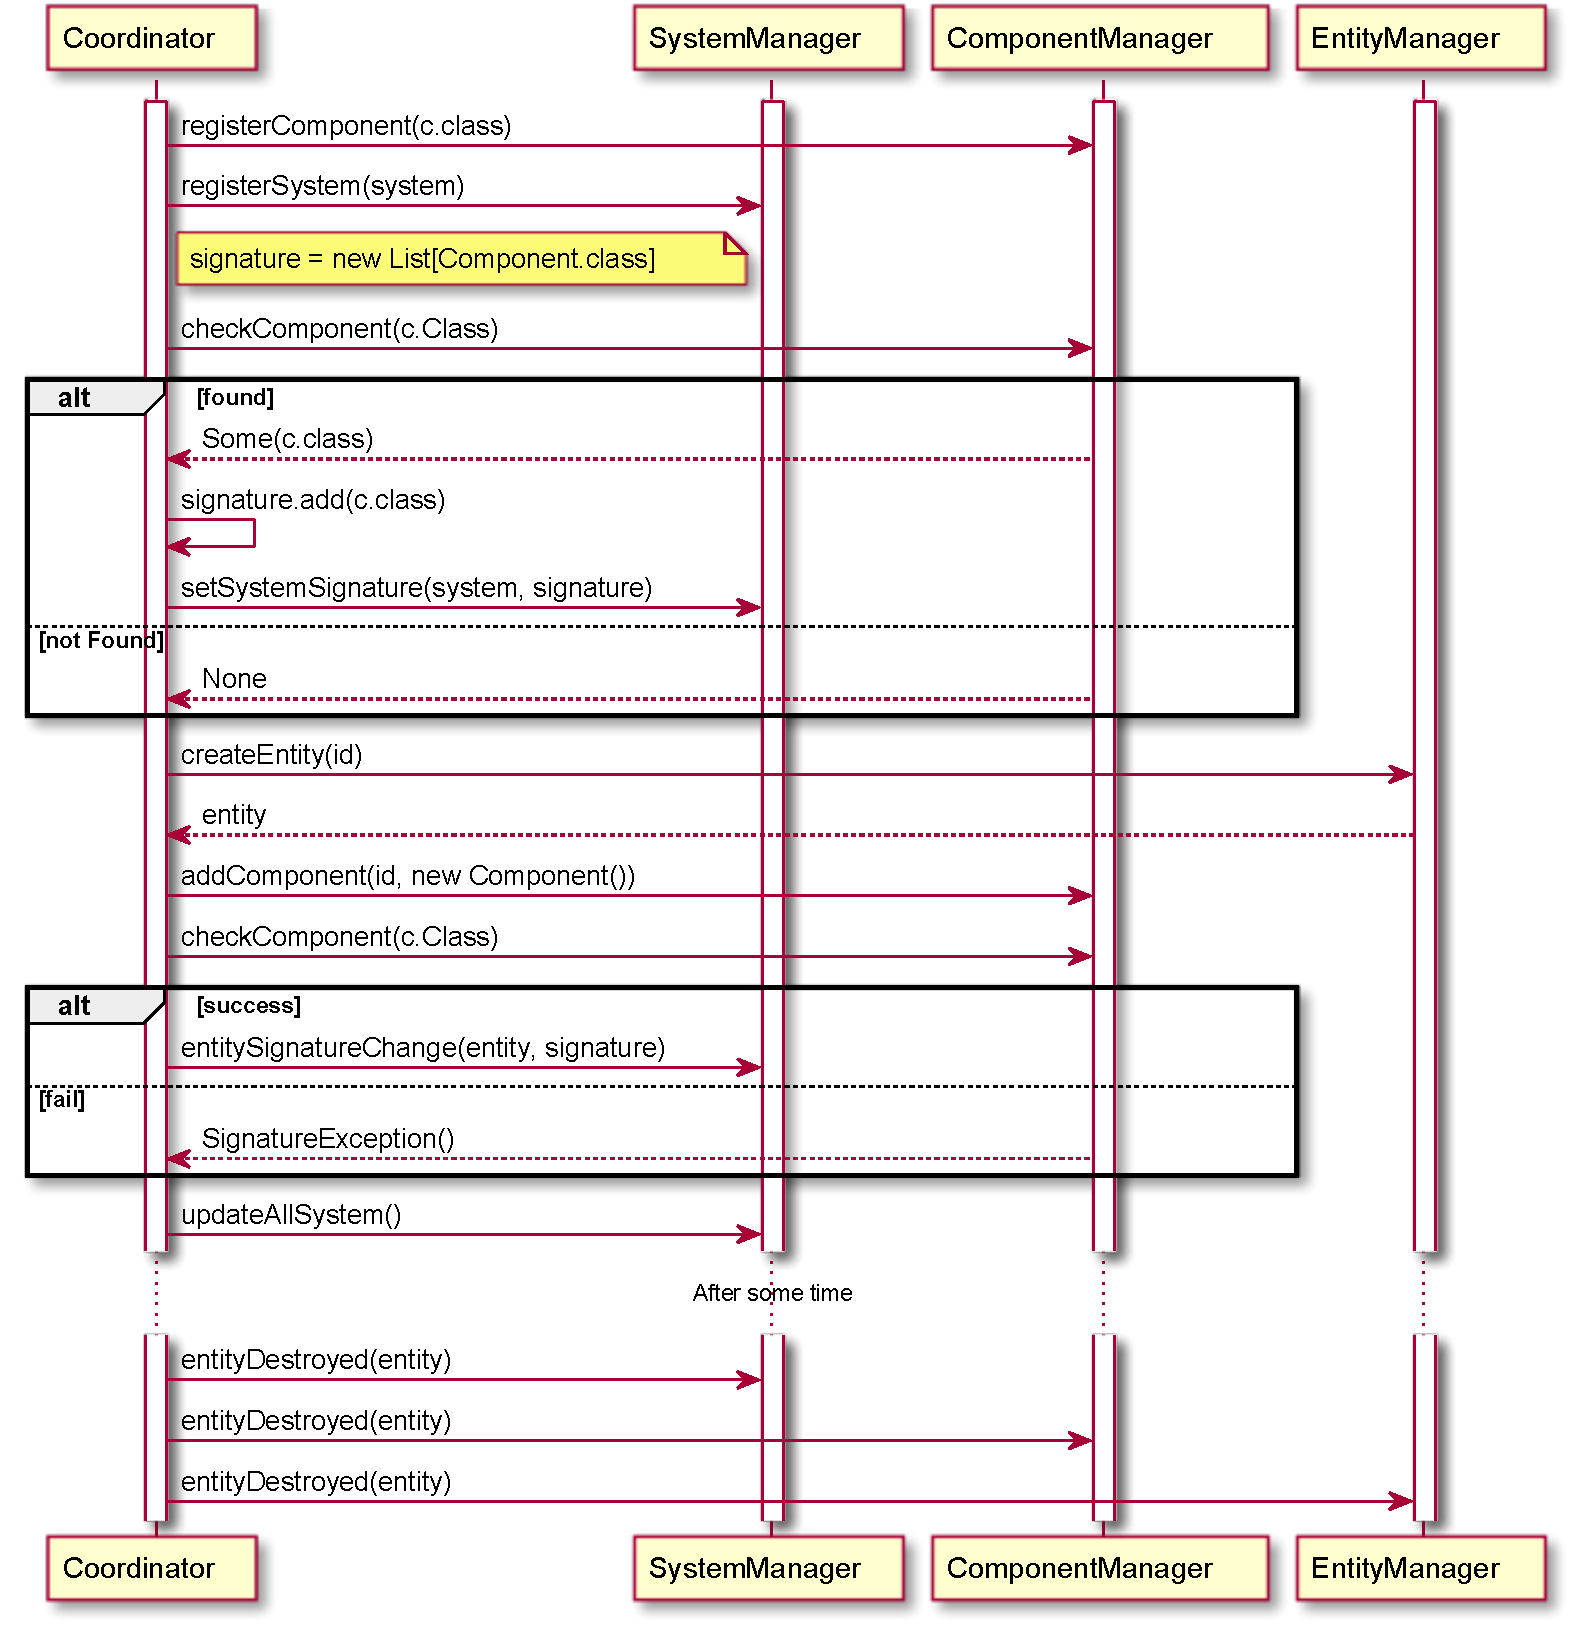
\includegraphics[width=0.99\columnwidth]{plantuml/rendered/sequenceDiagrams/sequenceECS.pdf}
	\caption{Diagramma di sequenza che mostra le varie interazioni fra gli elementi di design.}
	\label{fig:sequenceECS}
\end{figure}

Il diagramma in figura \ref{fig:sequenceECS} mostra le interazioni principali fra gli elementi in gioco. I passi fondamentali che vengono mostrati possono essere riassunti in pochi macro step:
\begin{enumerate}
	\item{\textbf{Registrazione dei componenti:}} un componente prima poter essere utilizzato deve essere \textbf{registrato} al \texttt{ComponentManager} in modo da \textbf{verificare} che non si utilizzino \textbf{componenti diversi} a runtime.
	\item{\textbf{Registrazione dei sistemi:}} successivamente è possibile registrare sistemi. La registrazione è molto semplice e consiste nell'assegnazione di una \texttt{Signature} al sistema. Una \texttt{Signature} non è altro che una \textbf{lista di tipi di componente} che definiscono la \textbf{natura del sistema}. Grazie a questo espediente è possibile delegare un sistema alla \textbf{gestione delle entità} a lui \textbf{compatibili}.
	\item{\textbf{Creazione di entità:}} in qualsiasi momento è possibile creare un'entità la cui \textbf{istanza} verrà conservata all'interno dell'\texttt{EntityManager}. È importante sottolineare che in questo caso l'entità non è ancora gestita da \textbf{nessun sistema} poiché \textbf{non possiede} componenti associati.
	\item{\textbf{Aggiunta di componenti ad entità:}} una volta che viene \textbf{associato} un componente ad una entità, l'entità potrà essere \textbf{assegnata} ai \textbf{sistemi compatibili} e quindi gestita.
\end{enumerate}
